\section{Introduction}
\label{sec:intro}
% Falar de metamodelacao muito por alto em Ecore e
% referencias para mais informacao sobre esta linguagem

Model transformation is the process of converting one or more input models to
one or more output models \cite{model_transformations} where each model
conforms to a metamodel (a set of well formedness rules that specify the abstract
syntax of models and the interrelationships between model elements, i. e., the
set of all possible conformant models \cite{unification_models}) specified using
a metamodeling language that in this case is \emph{Ecore}.

\emph{Ecore} is a subset of the \emph{Unified Modelling Language} (\emph{UML})
and the main language for the creation of metamodels in the \emph{Eclipse
Modelling Framework} (\emph{EMF}) \cite{emf_book}.

\emph{EMF} provides a modelling framework and code generation facility that lets us
define models, from which then we can generate other models or code for building
tools and other applications \cite{emf_book} \footnote{For more
information about the \emph{Ecore} language and \emph{EMF} refer to
\url{http://www.eclipse.org/modeling/emf/?project=emf}}.

Figure \ref{fig:model_trans_general} shows the model transformation process. We
can see that every model involved has to conform to some metamodel. At the
highest level, the metametamodel conforms to itself meaning that its structure
can be expressed with the same terms it describes. The rules that make
up the transformation process are also expressed in a model that is interpreted
by some engine that takes some input models and generates some output
models.

\begin{figure}[h]
\begin{center}
  \includegraphics[scale=0.6, trim=3.3cm 13.6cm 3.1cm 0.7cm,
  clip]{imgs/model_transformation.pdf}
  \caption{Model transformation process and required elements.}
  \label{fig:model_trans_general}
\end{center}
\end{figure}

\clearpage

\subsection{What is \emph{DSLTrans}?}

\emph{DSLTrans} is a language specifically designed to support the definition of
\emph{Ecore}-based model transformations \cite{dsltranslator}. It is particularly
useful when building a new language (for instance, a language to describe graphical
user interfaces) whose semantics are not known and it is necessary
to express them in terms of an existing well known language (a Java
application\footnote{Java code can be modelled using an \emph{Ecore}-based metamodel
thus making it possible to treat Java applications as models}).

The process of assigning meaning to a new language trough transformations
involves coming up with a set of mappings between the terms of the source
language to terms in the target language \cite{dsltranslator}. In \emph{DSLTrans} those
mappings are expressed in the form of rules where the first part of each rule
has a pattern describing some arrangement of terms in the source language and
the second part has the terms to be created in case the first part exists in
some input model.

Figure \ref{fig:model_trans_manual} shows the model transformation process
according to the technologies and tools used throughout this manual. As you can
see, \emph{DSLTrans} is a metamodel used to express transformations that are
interpreted by the \emph{DSLTranslator} engine to translate models.


\begin{figure}[h]
\begin{center}
  \includegraphics[scale=0.6, trim=3.3cm 13.6cm 3.1cm 0.7cm,
  clip]{imgs/model_transformation_dsltrans.pdf}
  \caption{Model transformation process and required elements used throughout
  this manual.}
  \label{fig:model_trans_manual}
\end{center}
\end{figure}

\clearpage

\subsubsection{A Metaphor}
\label{subsubsec:metaphor}
% Da um exemplo de transformacao, realcando a questao dos mapping 1-1. Tem
% informacao desta no manual do dsltrans.

In order to better understand all these concepts, lets focus on a simple example where
we have a small language (a.k.a. a metamodel) used to define an individual's genealogy tree and we will come up with transformations that present information from some genealogy tree (a.k.a. model) in different views.

Figure \ref{fig:genealogy_tree_example} shows an example of a genealogy tree. We
can see that John and Mary married and had one son: Thomas who in turn married
Sarah\ldots and so on.

\begin{figure}[h]
\begin{center}
  \includegraphics[scale=1, trim=4.1cm 17.4cm 4.1cm 3.6cm,
  clip]{imgs/genealogy_tree_example.pdf}
  \caption{Genealogy tree example.}
  \label{fig:genealogy_tree_example}
\end{center}
\end{figure}

How can we find out, given a tree of any size, who are the couples? More
specifically we want as a result of the transformation a set of couples like the
one shown in figure \ref{fig:couples_example}.

\begin{figure}[h]
\begin{center}
  \includegraphics[scale=1, trim=5.6cm 21.0cm 8.4cm 3.8cm,
  clip]{imgs/couples_example.pdf}
  \caption{Couples set example.}
  \label{fig:couples_example}
\end{center}
\end{figure}

The transformation rules have to be based on patterns as described earlier so
something like figure \ref{fig:gen_to_couple_example} should be fine. The
transformation is only made of a single rule, that says the following:
\emph{Every person that is married to other person in the source model becomes
the same person associated with the same other person in the target (or output) model.}
Notice that the connections in the source model are different
than those in the target model.

\begin{figure}[h]
\begin{center}
  \includegraphics[scale=0.9, trim=3.5cm 21.5cm 3.8cm 4.2cm,
  clip]{imgs/gen_to_couple_example.pdf}
  \caption{Genealogy to Couples transformation.}
  \label{fig:gen_to_couple_example}
\end{center}
\end{figure}


Another way of looking at the transformation is by defining two rules: one
establishing the fact that \emph{every married couple in the source metamodel becomes two
individuals in the target} and afterwards \emph{add} the relation between those
two individuals, forming a couple. Figure \ref{fig:gen_to_couple_example_extended} illustrates this approach. Notice that the dashed links between the source and
target model elements mean that in the bottom rule we don't want to create new
elements in the target model: we only want to create a connection between them.

Although partitioning the transformation and referring
to elements that already exist in the output model\footnote{because these elements where generated by some previous rule} may seem too much work and counter-intuitive; for complex transformations it is a more natural way since we start by looking only to each
element individually and expressing its meaning in the target language through simple rules, then we explore more and more complex patterns saying what those
mean.


\begin{figure}[h]
\begin{center}
  \includegraphics[scale=0.9, trim=3.5cm 17.0cm 3.8cm 4.2cm,
  clip]{imgs/gen_to_couple_example_extended.pdf}
  \caption{Genealogy to Couples transformation - Partitioned.}
  \label{fig:gen_to_couple_example_extended}
\end{center}
\end{figure}


\clearpage

\subsection{DSLTrans and Other Transformation Languages}
\label{subsubsec:other_languages}

There are several papers about transformation languages. Bellow is a brief description of some of them so you can have an idea about their general features with respect to \emph{DSLTrans}.


\subsubsection{QVT} 

Query / View / Transformation is a standard defined by the
\emph{Object Management Group}; its implementation is \emph{SmartQVT}: a
tool that compiles model transformations specified in QVT to produce Java code
used to perform these transformations \cite{qvt_transformation_language}.

\subsubsection{ATL} 

\emph{Atlas Transformation Language} is a transformation
language inspired by the \emph{QVT} requisites that uses the \emph{OCL}
formalism. It provides declarative constructs as we used in the previous example
and, for the most difficult transformations, it allows the user to define
imperative rules, which increases its flexibility and complexity
\cite{atl_transformation_tool}.

\subsubsection{ATC} 

\emph{Atomic Transformation Code} is a low level model transformation language
with the main purpose of being the target for other transformation
languages' specifications allowing for the execution of a diversity of model
transformation languages via translation to \emph{ATC} \cite{atc_user_guide}.


\subsubsection{ETC}

\emph{Epsilon Transformation Language} is an hybrid\footnote{ An hybrid transformation language is one that provides both imperative and
declarative constructs, as \emph{ATL}, \emph{ETC}, and others.}, rule-based model-to-model transformation language that has the flexibility of allowing for query, navigation and
modification of multiple target and source models \cite{epsilon_eclipse}.


\subsubsection{MOLA}

\emph{MOdel transformation LAnguage}, similarly to \emph{DSLTrans}, is a graphical
transformation language that strives to produce readable transformations by
combining traditional structured programming in a graphical form with simple
pattern rules \cite{mola_trans_language}.


\subsubsection{RubyTL}

\emph{Ruby Transformation Language} is a domain specific hybrid
transformation language embedded in Ruby that provides an extension
mechanism based on plugins \cite{rubytl}.

\subsubsection{UMLX}

\emph{UMLX} is a graphical transformation language that extends \emph{UML}
through the use of transformation diagrams that are no more than class diagrams
with additional relations to specify mappings between input and
output models \cite{umlx}.

\subsubsection{GReAT}

The Graph REwriting And Transformation is a rule-based graphical language that,
as DSLTrans, sees models as labelled graphs and uses graph
transformation formalisms to translate them \cite{great}.

\subsubsection{\textbf{DSLTrans}}

With respect to the described transformation languages, \emph{DSLTrans} is a
rule-based graphical transformation language\footnote{The latest version of DSLTrans supports also textual syntax for transformation specification} that uses declarative constructs and graph formalisms to prescribe transformations. A distinctive characteristic is that all the
transformations specified in \emph{DSLTrans} are guaranteed to terminate\footnote{DSLTrans
transformations are guaranteed to terminate because the language doesn't
support loop constructs and no rule can be applied forever. This means the
language is not Turing complete but there are techniques that allows us to
build complex and still readable transformations as you will see.}.
This means the language is not Turing complete and for very complex transformations it might not be the ideal transformation language.
% TODO Colocar aqui definicao de traducao e transformacao se o bruno responder ao email.



% TODO A brief history of DSLtrans
% \subsection{\emph{DSLTrans} Biography}


\clearpage

\subsection{Assumptions}

\subsubsection{User}

% Descreve as assuncoes que fazemos acerca do utilizador:
% - Sabe metamodelar . . . etc
About the reader of this manual and hopefully user of \emph{DSLTrans} we make
the following assumptions:

\begin{description}
  \item[Modelling Jargon] The reader should be familiar with the modelling terms
  like model, metamodel, metametamodel, model transformation, language,
  etc\ldots. \cite{unification_models} and \cite{model_transformations} give
  readable overviews of most of the terms used throughout this manual.
  \item[Eclipse Modelling Framework and Ecore] The user knows how to use the EMF
  main metamodeling language to created metamodels and respective instances. For
  more information refer to the project's home
  (\url{http://www.eclipse.org/modeling/emf/}) or read the EMF book in
  \cite{emf_book}. There is also a good tutorial on how to create
  metamodels here:
  \url{http://tinyurl.com/3oo8woz} 
  \item[Advanced System User] We assume that the user knows how to change
  environment variables and install software in its system.
\end{description}


\subsubsection{Environment}

% Descrever as caracteristicas exactas do software usado.
% - Deve ter uma indicacao precisa do sofware usado, nomeadamente, versao de
% eclipse e versao dos plugins do dsltrans.
In order to succeed in learning DSLTrans and following the examples presented in
this manual it is highly recommended that you have the following tools:

\begin{itemize}
  \item Eclipse Modeling Tools, Helios Service Release 2. You should be able to
  download it in the eclipse home page \url{http://www.eclipse.org}. After
  starting eclipse and going to \emph{Help, About Eclipse}, you should see the
  version info shown in figure \ref{fig:rec_eclipse_version}.
  \item SWI-Prolog version 5.10.4 by Jan Wielemaker. The \emph{DSLTranslator}
  engine uses the Prolog language internally to process the transformations. You should
  be able to download SWIProlog from the project's home page
  \url{http://www.swi-prolog.org/}. Figure \ref{fig:rec_prolog_version} shows
  Prolog's version info.
\end{itemize}


\begin{figure}[H]
\begin{center}
  \includegraphics[width=0.9\textwidth]{imgs/eclipse_version.jpg}
  \caption{Recomended eclipse version.}
  \label{fig:rec_eclipse_version}
\end{center}
\end{figure}

\begin{figure}[H]
\begin{center}
  \includegraphics[width=0.9\textwidth]{imgs/prolog_version.jpg}
  \caption{Recomended prolog version.}
  \label{fig:rec_prolog_version}
\end{center}
\end{figure}


\begin{comment} 

Eclipse:
	Eclipse version: Eclipse Modeling Tools Helios Release
	
	Plugins:
		dsltransAnalysis_1.0.0.201107201833.jar
		DSLTransEditor.diagram_1.0.0.201008111406.jar
		DSLTransEditor.editor_1.0.0.jar
		DSLTransEditor.edit_1.0.0.jar
		DSLTransEditor_1.0.0.jar
		DSLTranslator_1.0.2.jar
		mprolog_1.0.0.201107201759.jar
		text_1.0.0.jar
		Transformer2.0_1.0.2.jar

WINDOWS:
	SWI Prolog version 5.10.x
	
		
LINUX:

			

\end{comment}

\clearpage

\subsection{About this Manual}


\subsubsection{Objectives}

After reading this manual the user should be able to:

\begin{itemize}
  \item Create and read \emph{DSLTrans} transformations either from scratch or by using
  prototyping techniques.
  \item Understand how higher order transformations work and even
  better: create them.
  \item Understand the advantages and limitations of \emph{DSLTrans} and
  when to use it instead of other transformation languages like ATL
  \cite{atl_transformation_tool}, \emph{SmartQVT}
  \cite{qvt_transformation_language} or others presented in page
  \pageref{subsubsec:other_languages}.
\end{itemize}


%\subsubsection{Notations}

% TODO Falar um pouco sobre as notacoes usadas no manual, estrutura, etc \ldots

\subsubsection{Structure}

% TODO O leitor deve ler com atencao a seccao de quickstart pois eh altamente
% recomendada e ensina muito!
If you are new to \emph{DSLTrans}, you should read
this manual from the beginning to at least section \ref{sec:language_def}. The
first sections are the ones that will help you understand the main concepts
behind the \emph{DSLTrans} and the remaining can be used as a reference.

This manual is divided in five sections:

\begin{description}
  \item[Installation] Where you will learn how to get the needed
  tools up and running so that you can follow the rest of this manual's examples
  and tutorials.
  \item[Quick Start] This section presents a hands on approach to
  \emph{DSLTrans} with a tutorial on how to create the transformation described
  in section \ref{subsubsec:metaphor} in two different ways. While it teaches
  you how to use \emph{DSLTrans}, it explains the main concepts and procedures
  involved in the creation of a transformation.
  \item[Language Definition] Where each element of a transformation is described
  and some examples in both graphical and textual syntax are given to help you
  understand how it can be used; possible restrictions and good practices are
  present. This section can be used as a reference as it contains the
  description of every element in the language.
  \item[Advanced Topics] Once you know how to use \emph{DSLTrans} well enough
  you will want to avoid some repetitive tasks when building most of the
  transformations. Since \emph{DSLTrans} is a metamodeled language it is
  possible to use it to transform transformations. This section focusses in
  teaching you how to use (and build) higher order transformations and to build
  complex transformation to simulate the stepping of abstract machines and even
  how to create transformations that are specific to some domain.
  \item[FAQ] Frequently asked questions and common errors are
  answered here.
\end{description}

\clearpage